% !TEX root = ../main.tex
\chapter{Method}
\label{ch:method}

\subsection{Experiment of this project}
In the context of this project, the observation is that current models are typically continuous (due to back-propagation), but many control tasks are not. An example of this is the problem of the pendulum with a fixed joint above and a loose joint below, which is swung up in a first step and then stabilized in the second step. When attempting to approximate the function that models this task, it becomes apparent that the function is not continuous. Due to the two distinct tasks involved, the agent must be able to recognize when the first task is complete and the second one begins. In the real world, there are many control problems that are not continuous.
The hypothesis is that discontinuous models would have an advantage in addressing these tasks. To test this hypothesis, multiple individuals can be evaluated in the environment (by going through the fitness function) and analyzing their performance, the number of individuals that solve the task, and other metrics. Hyperparameters also play an important role in improving the performance of individuals in the environment.

\section{Fitness}

The fitness class serves as an interface between the model and the environment. It implements the control loop at its core, through the $fit$ function.
The control loop essentially evaluates how well a set of weights performs in an environment by selecting actions, as determined by the model, and outputting a score based on its performance.

\begin{algorithm}
\caption{fit}
\label{pseudo_fit_function}
\begin{algorithmic}[1]
\State reset the environment and get the observations
\State set the weights of the individual in the model
\State score = 0
\State done = False
\For{number of step $nsteps$}
    \State get the action given from the model and the actual observation
    \State execute an action step and get the state of the environment
    \State increment the score with the obtained reward from the action step
    \If{done}
    	\State break
    \EndIf
\EndFor
\Return score
\end{algorithmic}
\end{algorithm}


\section{Environments}

For this project, two environments of the $Box2D$ category of OpenAI Gym were used\footnote[1]{https://www.gymlibrary.dev/environments/box2d/}. These environments are more complex than the "Classical Control" problems and are highly configurable. Box2D is a 2D physics engine for games that can be used to make objects move in a realistic way and make the game more interactive.(\cite{noauthor_box2d_nodate}).

\subsection{Lunar Lander}
The Lunar Lander environment consists of a rocket attempting to land between two flags on the surface of the Moon. The rocket can use three engines, which can be fired at full speed or turned off. The environment has both a continuous and a discrete version. For this project, the discrete version was used. Figure~\ref{fig:lunar_lander} illustrates the different states in which the rocket can be during the landing.
\begin{figure}[!ht]
\centering
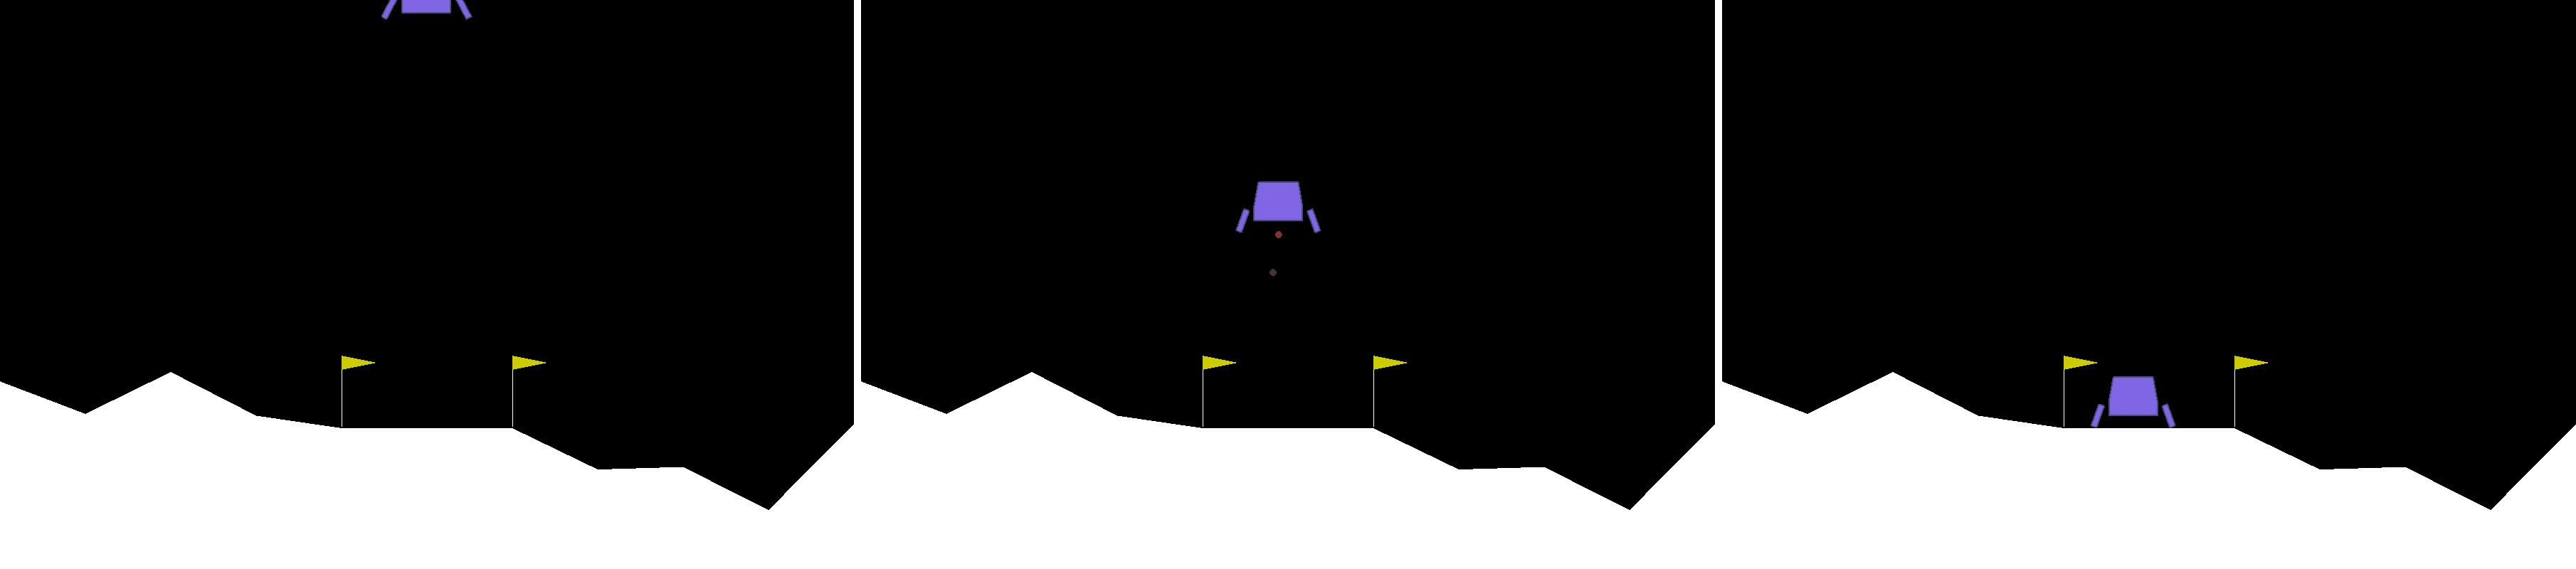
\includegraphics[width=1\textwidth]{lunar_lander}

\caption[Lunar Lander illustration]{
  \textbf{Different states of the Lunar Lander environmment}
The left image illustrates the rocket at the beginning of the task. The image in the middle shows the rocket firing its main engine in order to adjust its trajectory and the right image shows a successful landing between the two flags.
 }
\label{fig:lunar_lander}
\end{figure}
\subsubsection{Action space}
The environment has four actions that can be used. It can either do nothing or fire with the engine on the left, on the right or the main engine, which points downwards. The power at which the engines fire cannot be adjusted (it can only be turned on or off). This means the action space is of dimension 4 and discrete.

\subsubsection{Observation space}
The observation space for the Lunar Lander contains eight values.
Two of them are booleans that indicate whether the corresponding leg of the lander is touching the Moon's surface or not, while all the other values are continuous.

\begin{table}[!ht]
\centering
\begin{tabular}{|l|l|l|}
\hline
\textbf{Observation} & \textbf{Min} & \textbf{Max} \\
\hline
coordinates of the lander in x & -1.5  & 1.5  \\
\hline
coordinates of the lander in y & -1.5  & 1.5  \\
\hline
linear velocity in x           & -5.0  & 5.0  \\
\hline
linear velocity in y           & -5.0  & 5.0  \\
\hline
angle                          & -3.14 & 3.14 \\
\hline
angular velocity               & -5.0  & 5.0  \\
\hline
left leg touching ground       & 0     & 1    \\
\hline
right leg touching ground      & 0     & 1   \\
\hline

\end{tabular}
\end{table}

\subsubsection{Rewards}
For the agent, starting from the top of the screen and successfully landing on the landing pad, it receives a reward of 100-140 points. If the rocket crashes, it receives a negative reward of -100 points. Touching the legs of the lander to the ground gives an additional reward of +10 points per leg and firing the engine gives a small penalty. The task is considered solved when the agent receives a total reward of 200 points or higher.It's worth noting that the rewards points may vary depending on the specific implementation of the environment, and that the exact points given for each action, state or event are not fixed values but can be adjusted to fine-tune the agent's behavior.

\subsection{Bipedal Walker}
This environment simulates a two-legged robot attempting to walk as far as possible on uneven terrain. Two versions are available: a "normal" version and a more challenging "hardcore" version which includes obstacles. The robot is composed of a hull and two legs, each with two joints, one connecting to the hull and the other allowing the leg to bend. Figure~\ref{fig:bipedal_walker} illustrates the robot in action on both versions.
\begin{figure}[!ht]
\centering
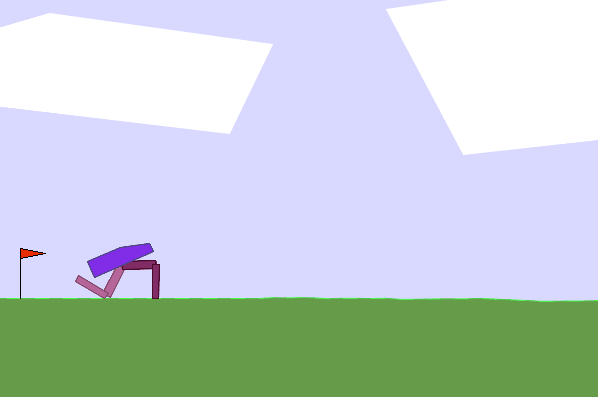
\includegraphics[width=1\textwidth]{bipedal_walker}

\caption[Bipedal walker illustration]{
  \textbf{Bipedal walker walking in both versions of the environment}
The left two frames illustrate the bipedal walker in different positions in the "normal" version of the environment. The right two frames show the robot attempting to walk over the obstacles in the "hardcore" version.
 }
\label{fig:bipedal_walker}
\end{figure}
\subsubsection{Action space}
The actions of the bipedal walker are continuous. There are four actions that can be performed, one for each joint. The values range between -1 and 1 and indicate the motor speed values of the corresponding joint. Each action affects the movement and stability of the robot, allowing it to walk or fall. The range of values can be adjusted depending on the implementation of the environment.

\subsubsection{Observation space}
The observation space for the bipedal walker is of dimension 24 and contains continuous values, except for the booleans that indicate whether the legs are touching the ground or not. The observation space contains information such as the angle and angular velocity of each joint, the linear velocity, and the position of the torso, among others.
Note that the position of the robot is not explicitly provided in the observation space, but it can be inferred from the other observations, such as the linear and angular velocities of the joints.

\begin{table}[!ht]
\centering
\begin{tabular}{|l|l|l|}
\hline
\textbf{Observation} & \textbf{Min} & \textbf{Max} \\
\hline
hull angle speed                    & -3.14 & 3.14 \\
\hline
angular velocity                    & -5.0  & 5.0  \\
\hline
horizontal speed                    & -5.0  & 5.0  \\
\hline
vertical speed                      & -5.0  & 5.0  \\
\hline
position of joints                  & -3.14 & 3.14 \\
\hline
joints angular speed                & -5.0  & 5.0  \\
\hline
left leg contact with ground        & 0     & 1    \\
\hline
right leg contact with ground       & 0     & 1    \\
\hline
10 lidar rangefinder measurements   & -1.0  & 1.0  \\
\hline

\end{tabular}
\end{table}

\subsubsection{Rewards}
A reward is given to the robot when it is able to move forward without falling. Falling is defined as the hull touching the ground and it is penalized by -100 points. If the bipedal walker reaches the end of the environment, it accumulates 300 points. Each time the robot moves its joints, it also receives a small penalty. The "normal" version is considered solved when 300 points are earned within 1600 time steps. For the "hardcore" version, the same amount of points has to be earned within 2000 time steps. The goal is to achieve the highest possible reward while avoiding falling and moving as efficiently as possible. Like for the Lunar Landar, the values can be adjusted to fine-tune the agent's behaviour.


\section{Model}
n this project, binary trees are employed as a model architecture instead of traditional neural networks. The optimization of these models is done using black-box optimization techniques. One of the advantages of using binary trees is their interpretability, as it is easier to understand the logic behind the decision-making process and explain the reasoning behind the model's predictions.
\subsection{Node}
A node in the binary tree is composed of a pointer that points to its parent node, a function that is part of the function class. The function applied at the node is used to make a decision or perform a computation based on the input data. An amount of weight the node contains, which is used to adjust the importance of the decision or computation made at that specific node. Lastly, two pointers, one to its left child and the other to its right child, which are used to navigate through the tree and make decisions based on the input data and the function applied at each node. Figure~\ref{fig:node_composition} illustrates a tree with a single node.
\begin{figure}[!ht]
\centering
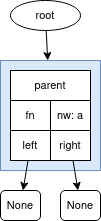
\includegraphics[width=.2\textwidth]{node}

\caption[Components of a single-node tree]{
  \textbf{Components of a single-node tree}
This represents a binary tree with a single node. The $root$ pointer points to the node, and the $parent$ pointer points to nothing as it is a single-node tree. The main components of the node are a function $fn$ that is implemented in the function class, an amount of weights $nw$ it contains, and two pointers to its left and right child ($left$, $right$) which point to None in this case.
 }
\label{fig:node_composition}
\end{figure}

\subsection{Functions}
Each node in the binary tree structure contains a function that is used to make decisions or perform computations based on the input data. In this project, three function types were implemented: a constant function, a linear function, and a perceptron.
The constant function returns the weights as output, regardless of the input values. The linear function returns the dot product of the weights and the observations it received as input. The perceptron uses a specific activation function, in this case the sigmoid,
\begin{equation}
1 \div(1 + \exp(-x))
\end{equation}
to transform the dot product between the weights and the observations (noted as $x$) into a scalar value that can be used to perform computations. Each instance of the function class contains a number of inputs and outputs, the weights used by the function, and the number of times the function was activated. The weights can be learned or fixed, and the input and output values can take a specific range.
Note that for nodes in the tree that are not leaf nodes, it is convenient to use linear functions as the output will be a scalar value that is useful for the traversal of the tree. The specific details of how the functions, weights and pointers are used to make decisions or perform computations in the tree, can be found in the activate function in \ref{binary_tree}. 

\subsection{Binary tree}
\label{binary_tree}
A binary tree is made up of linked nodes that contain functions. Figure~\ref{fig:tree_composition} illustrates a binary tree with a root node and two child nodes.
\begin{figure}[!ht]
\centering
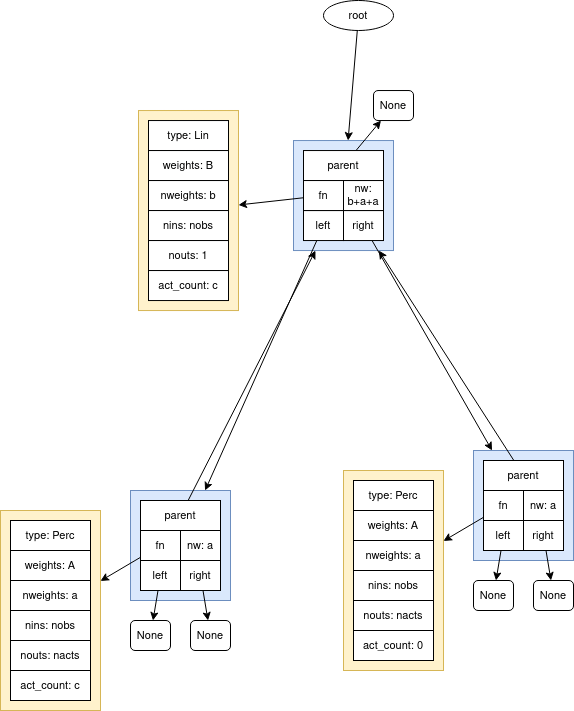
\includegraphics[width=.6\textwidth]{tree}
\caption[Components of a tree with three nodes]{
  \textbf{Components of a tree with three nodes}
Representation of a tree with a root node containing a linear function and two child nodes with perceptrons. Each node shows its pointer to the corresponding function instance (yellow blocks) and the links to each other. The $n$ before variables or values stands for "number," thus $nobs$ means the number of observations, for example.
 }
\label{fig:tree_composition}
\end{figure}
A binary tree is a structure composed of linked nodes that contain functions that are used to make decisions or perform computations based on the input data. Each node in the tree has a function, which can be one of the types implemented in the project (constant function, linear function, perceptron) and two child nodes that can be either leafs or internal nodes.

The process of using the tree to make decisions or perform computations is known as activation. The activate function starts from the root of the tree and navigates through the tree by following the links between the nodes based on the output of the function of the current node. When it reaches a leaf node, it returns the output of the function of that node as the final output of the tree.

The construction of the tree is done by deciding the decision points in the tree, these decision points are chosen based on the problem to solve and the input data. The tree can be trained and updated by adjusting the functions, weights, and links between the nodes.

The binary tree has some advantages and limitations when compared to other models such as neural networks and decision trees. One of the advantages is that it can be interpretable, as the decision points and functions used in the tree can be explained. However, one of the limitations is that it can be sensitive to the size of the tree, making the efficiency of the tree depend on the size of the tree. This can be overcome by applying pruning techniques or other methods to optimize the tree structure.
\begin{algorithm}
\caption{$activate$ function}
\label{activate function}
\begin{algorithmic}[1]
\State starting from the root
\While{true}
\If{$node$ is a leaf}
    \Return output of $node$'s function 
\ElsIf{output of $node$'s function > 0}
    \State go to the left child node
\Else 
    \State go to the right child node
\EndIf
\EndWhile
\end{algorithmic}
\end{algorithm}
The difficulty of tasks can vary, making it important to have the ability to adjust the size of the tree accordingly. For instance, simpler problems like the Cartpole in OpenAI Gym can be solved with a small tree, while more complex problems require a larger tree. Increasing the size of the tree allows for more complex decision making and can improve the model's performance. However, it also increases the risk of overfitting.
In this project, a function has been implemented to automatically increase the size of the tree as the difficulty of the problem increases. This process of finding an optimal structure is known as architecture search. The implemented function illustrates only one of many possible techniques for increasing the tree structure.

The function works by randomly selecting a leaf node and adding two new nodes to it. It starts by traversing the tree randomly until it reaches a leaf node. Then, it checks if the selected leaf is the root of the tree or not. If it is the root, a new parent node is created, otherwise, the leaf's parent node is copied to create a new parent node. The new parent node is then set as the parent of the current leaf node and its copy. The new nodes are added to the tree in such a way that the relative position of the current leaf node to its previous parent node remains the same.

It is important to note that the function does not add two child nodes to the leaf node, but one new node is added as the parent of the leaf node and the other as its sibling. Figure~\ref{fig:add_node} illustrates an example of adding two nodes to a binary tree. After the addition of the new nodes, all the links in the tree need to be fixed and the information about the number of weights and the amount of descendants needs to be updated. To accomplish this, the function uses a propagation of the information from the current leaf node to the root.
\begin{figure}[!ht]
\centering
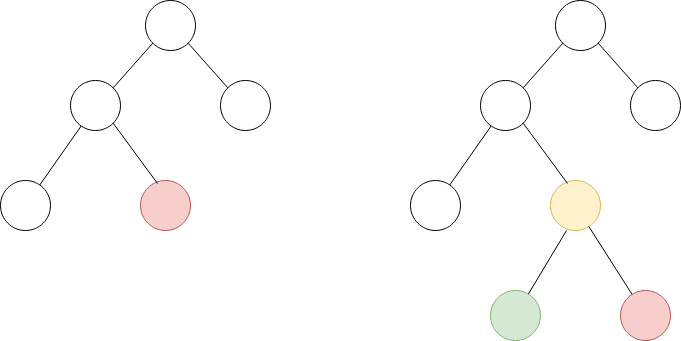
\includegraphics[width=.6\textwidth]{add_node}
\caption[Addition of two nodes in a binary tree]{
  \textbf{Addition of two nodes in a binary tree}
  The left tree shows the initial tree before the addition of the nodes. The red node represents the randomly chosen leaf from which the node addition will follow. The tree on the right represent the tree after addign two nodes with the $add_node$ function. The node in yellow is the newly created parent node and the green node is the sibling of the previously existing red node. Notice that the red node keeps its relative position to the parent node.
 }
\label{fig:add_node}
\end{figure}
\begin{algorithm}
\caption{$add\_node$ function}
\label{add_node function}
\begin{algorithmic}[3]
\State pick a random leaf
\If{leaf is a root}
    \State create $new\_parent$ node (root) with a linear function
\Else
    \State copy leafs parent into $new\_parent$ node
\EndIf
\State create $copy\_node$ (copy of leaf)
\State set $copy\_node$ and leaf as children of $new\_parent$
\State fix links
\State propagate the count of new nodes and their weights up the tree
\end{algorithmic}
\end{algorithm}

The function for increasing the size of the tree allows for the tree to adapt to the difficulty of the problem by growing according to a stagnation threshold, where the score of the individual does not improve for a certain number of steps. A larger tree has a larger search space, which allows it to solve more complex problems. However, it also increases the computation time. Therefore, it is important to find the right balance between growing the tree too quickly or too slowly.